\label{ch:theory}
\TLSAY{please use a spell checker, there are many typos in your text} 

In this chapter\TLINS{,} \TLDEL{all} the fundamental theory, metho\TLINS{do}logy and protocols used in this implementation are \TLREP{ elaborated}{introduced}. This is meant to serve as a tool to aid in an intuitive understanding to further clarify the design and its underlying choices\TLSAY{what? this sentence makes no sense to me}. As stated PDD is the research of which this thesis is based\TLSAY{PDD is a methodology not a research}.  Before delving in to the theory it is important to clarify what \textit{Interval Property Checking} (IPC) is and how it can be used to create a sound relationship between the two abstraction layers with \textit{Path Predicate Abstraction} (PPA). In \TLSAY{Use Sec.~\ref{sec:ipc} instead of section ref, everywhere}  section \ref{sec:ipc} IPC is described together with necessary additional information. What PPA is and how it is used to bridge the semantic gap is covered in section \ref{sec:ppa}. Section \ref{sec:pdd} then explains PDD and the certain rules it imposes on the ESL descriptions. Finally the AMBA-AHB specification is reviewed in section \ref{sec:ahb}.       


\section{Interval Property Checking}
\label{sec:ipc}
Formal verification is an approach of functional verification where design specification is formally formulated as a set of properties. Using mathematical algorithms \TLSAY{use active not passive ... who is it? a property checker proves ... } \TLSAY{browse your text, don't always use may/can/could .. it is proven, that}  it can be proven that the RTL description fulfills the property set. As opposed to simulation based RTL verification, formal verification can\TLSAY{can it or can it not?} guarantee the absence of bugs in the design. Recent industrial languages such as \textit{Interval Language} (ITL) provide an intuitive alternative to formulate such properties using a formal language such as \textit{Linear Temporal Logic} (LTL)\TLSAY{LTL is not a language is a theory}. An interval property, or operation property \TLSAY{with the difference between an IPC property and an operation property?} \TLSAY{Make more use of paragraphs}  is a pair of assumptions $A_t0$ and commitments $C_t1$. The assumptions describe the state and inputs of some RTL cluster over a time $t_0$ whereas the commitments describe the state and outputs of the same RTL cluster over time $t_1$. Using a property checker one attempts to prove that if the assumptions hold on the design, the commitments do as well. Here the time variables $t_0$ and $t_1$ represent a a time period relative to an arbitraty timepoint $t$. The property structure is illustrated in figure \ref{fig:exop}.  

\begin{figure}[hbt]
\begin{lstlisting}
  property grant_master is
    assume:
       at t: some_state;
       at t: request_signal;
       at t+1: grant_signal;

    prove:
       at t+2: another_state;
       at t+2: not(request_signal);
       at t+2: address_signals;
  end property; 
\end{lstlisting}
\label{fig:exop}
\caption{Example operation property}
\end{figure}

Starting from all possible starting states the property checker searches for an input sequence and a path in the \textit{Finite State Machine} (FSM) where the implication of the $A_t0$, $C_t1$ pair does not hold. The property checker used in this thesis is Onespin 360 DV, or Onespin for short \cite{onespin}. 

\subsection{Complete Interval Property Checking (C-IPC)}
\label{subsec:cipc}
A set of properties only guarantee that the design works according to specification if the appropriate termination criterion is used. This criterion was first defined in \cite{bormannbusch}. For a property set to qualify as complete some conditions must be fulfilled. The idea is that, starting from reset there are property \TLSAY{is are property properties?} covering every aspect of the I/O behaviour and transitions through all important states of the design. The termination criterion hereby referred to as completeness is checked using the property checker Onespin. \TLSAY{Before you can explain what the checker does explain what is actually checked, completeness is not really about the property graph}  A completeness check is not run automatically on the design, rather a completeness description must be manually created. This description contains all inputs, determination requirements (outputs, state variables) and a property graph connecting the properties as a FSM \TLSAY{As a property graph} . It is not generated automatically to help detect faults in the property set rather than having them transferred to the completeness description. The design behaviour can be guaranteed by a series of tests.
\begin{enumerate}
 \item \textit{Reset test}: It is proven that reset can be applied deterministically and that all outputs and state variables are determined after reset based on listed assumptions.
 \item \textit{Successor test}: Proves that the assumptions of all properties are either inputs or state variables determined by a preceding property. All properties must be properly hooked together, meaning that all assumptions (except inputs) in a property at time $t$ (left hook) is determined by all predecessing properties at the same timepoint (right hook). This ensures there are no gaps between properties where signals are undefined. 
 \item \textit{Determination test}: Proves that all state variables are determined at the right hook in every property, and that all relevant outputs are determined at all times. Relevant in this context is meant by the validity of certain data. In communication data may be invalid unless f.ex a flag is set, the completeness checker can be told to ignore this value otherwise by describing it as \textit{if(flag) then determined(data)}.
 \item \textit{Case split test}: Proves that there is a property covering every transition between important states of the design. In other words there is a property covering every input scenario in every important state. 
\end{enumerate}

As long as only inputs are listed as inputs in the completeness description, and all outputs are listed as determination requirements, the collective hold of all four tests prove completeness. Out of sheer relevance to this thesis key aspects of the process on how to achieve completeness on a design is provided in the following section. 

\subsection{Gap Free Verification}
\label{subsec:gfv}
Out of consistency some terms from the previous section are redefined. A state variable is redefined as a \textit{Visible register}. It is a register \TLSAY{is it really a register? in case of forwarding this is not the case ... it's more like a symbolic register} that stores information used between properties. It is not necessarily used to determine the state of the system. This is where the term \textit{Conceptual state} comes in. Earlier referred to as important states, conceptual states are abstractions of actual states in the designs FSM \TLSAY{why not stick to important states, if it is the same thing?}. It may directly map to a state in the FSM, parts of one,  contain many or be a collection of visible registers and inputs of a design. The process of creating a property set that proves completeness is divided in four phases. The specifics of the four phases will not be recounted here, for that the reader is referred to \cite{gapfree}. Rather some implications and key information are re-described. \\
\newline 
\TLSAY{A paragraph is enough you don't always need a new line} 
The process starts with the definition of the \textit{Conceptual State Machine} (CSM) and a set of skeleton properties are made to represent this CSM in the property graph. All visible registers required to correctly represent the assumptions of the properties are added as local determination requirements and determined at right hook in all properties. By making sure all properties only assume inputs and these registers (at correct timepoint) the successor test will hold. Further, all outputs are listed as determination requirements together with the remaining visible registers needed to help determine them, they are subsequently determined in all properties. If this is done correctly the determination test will hold. Outputs are only determined based on inputs and visible registers. If the mapping of a visible register is incorrect or missing, this is sure to appear as an error in the completeness check. If all possible transitions of the CSM is covered by properties, the case split test will hold. If not, these operations are identified with help of the debugger and added until the case split test holds. The reset test is just a special case of these three tests, and is unlikely to fail if all three hold\TLSAY{I don't think this is true}. When all four tests hold the property set is complete. 

\subsubsection{Clusters}
\label{subsub:clust}
\TLSAY{What is a cluster?}
A design is ideally verified in a single cluster, to keep abstraction at the highest level. In some cases verifying a design in a single cluster is not feasible. The main reason for this is parallelism.\\ 
\begin{wrapfigure}{l}{5.5cm}
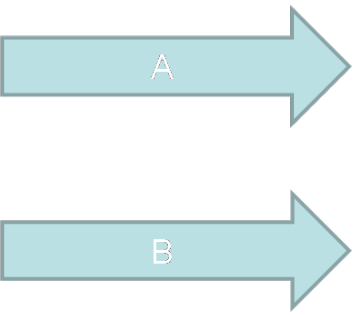
\includegraphics[width=5.5cm]{figs/Verif/parallell.png}
\caption{Parallel dataflow}\label{fig:para}
\end{wrapfigure} 

Consider two dataflows occuring in parallel. To verify this completely, every scenario must be accounted for. A gets data and not B, B gets data and not A, both A and B or neither. This needs to be accounted for in every clock cycle. In a large design with many operation properties, verification becomes unfeasible even with two parallel data flows.     


Where one draws the conceptual border of a cluster, often falls naturally on the interface between to modules. Sometimes however, it is necessary to do a cluster split where the border consists of arbitrary signals in the middle of a module. Any signal can be determined as an input or output to the completeness plan of a cluster\cite{clust}. When splitting a design into clusters it is important to verify all clusters completely and that any signal that is defined as an input to a cluster is either an input to the design, or an output from another cluster. When defining the signals that represent inputs and outputs between clusters it is recommended to use the same signal names in both clusters. An example of this is using the top level signal in the RTL design that connects cluster A to cluster B. This is to eliminate the possbility that an output from cluster A actually represent a different signal than its respective input to cluster B. By following these guidelines there are no gaps in verification between the clusters. 



\section{Path Predicate Abstraction}
\label{sec:ppa}

This section reviews the principles of PPA and how it is used to describe RTL at a higher level of abstraction using operation properties. \TLREP{it}{It} provides   \TLSAY{PPA does not describe the RTL means for abstraction} This does not serve as a standalone description of the full theory, for that the reader is referred to \cite{2014-UrdahlStoffel.etal}. To give an intuitive understanding of the abstraction mechanism PPA is discussed with regard to FSM's. Consider an arbitrary RTL design and its accompanying FSM. This FSM has its own input and output alphabet and describes a possibly complex sequence of operations. PPA is used to simplify this sequence of operations by identifying only the important states, a process illustrated with operational graph coloring. \\ 

\begin{figure}[hbt]
\label{fig:ppa}
 \centering
 \begin{subfigure}[b]{0.4\linewidth}
 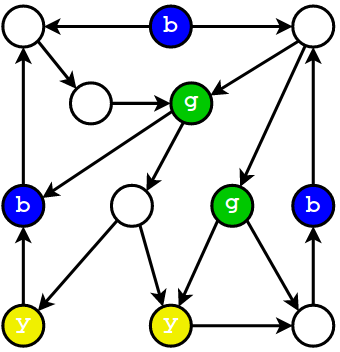
\includegraphics[width=\linewidth]{figs/opcoloring.png}
 \caption{Operationally colored graph}
 \end{subfigure}
 \begin{subfigure}[b]{0.3\linewidth}
 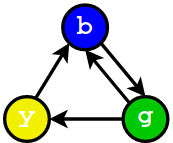
\includegraphics[width=\linewidth]{figs/ppa.png}
 \caption{Resulting PPA}
 \end{subfigure}
\end{figure}

With operational coloring one is able to choose quite freely which states to group together in a conceptual state, and which to leave out as "unimportant" states as long as two rules are followed. 
\begin{enumerate}
 \item All cyclic paths must be broken by at least one colored node, there must be no cyclic path in only uncolored nodes. 
 \item If there is a path between two colored nodes $g\rightarrow y$, there must exist a path to a node of color $y$ from any node of color $g$. 
\end{enumerate} 

Figure \ref{fig:ppa} a) shows the operationally colored FSM of the RTL and b) shows the resulting PPA. It can be easily verified that the color sequence of any path in a) is represented in b). Through abstraction the FSM has been greatly simplified, although some information is lost in the process. It is not possible to extract the original FSM based on the abstraction. An accompanying abstraction of the input and output alphabet of the original must be derived. A communication spanning several nodes in the FSM can now be represented using a single compound in one transition. What before was SDRAM controllers \textit{burst\_read} spanning or 8 more cycles can now be represented as a single operation with $sdram\rightarrow read(compound)$. All transitions between the nodes of the PPA together with the abstract input and output alphabet are formulated in operation properties. This set of properties can now be refined to hold on the original design, and a completeness analysis can be run. As covered in section \ref{subsec:cipc} this verifies the complete I/O behaviour of the design, and the set of abstract properties can be said to be a sound abstraction of the RTL.  



\section{Property Driven Development}
\label{sec:pdd}
\TLSAY{Maybe you can try and explain at least what the connection between SystemC, SystemC-PPA and RTL is? This feels really into detail} 
In this section the idea of PDD is described, with the intention of giving an overview of how two cycle accurate communicating RTL modules can be abstracted to an untimed ESL description. For a complete overview of the design flow, case studies and proofs the reader is referred to \cite{pddref}. \TLSAY{Add some paragraphs} Instead this section focuses on the abstraction of communication and what restrictions this puts on the implementation language; SystemC. In the previous section properties were manually described bottom-up based on an existing RTL description. With PDD this process is reversed (top-down) and properties are automatically generated from an ESL description written in this restriced subset of SystemC, referred to as SystemC-PPA. The RTL is then designed based on these properties, in a process similar to test driven development in software. A software tool \textit{DeSCAM} \cite{descam} analyses the SystemC-PPA and a complete set of properties representing design behaviour can be printed.\\
\newline
A system model consist of multiple units transferring information between each other by some means of communication. Communication at the hardware level is divided in two main categories, asynchronous and synchronous. In asynchronous communication transmission is enabled through event signaling, where the receiving end must always be ready to receive such an event. Synchronous communication is enabled through use of a common clock, it is understood through explicit timing that the receiver is ready. There is also the case of unilateral synchronization, where only one communication partner sends such an event. It must then be guaranteed through timing that the other partner is ready. The abstract system model consists of asynchronous PPA's which communicate with eachother using events. In SystemC-PPA \TLREP{this communication is done over}{communication is implemented with} channels using port interfaces. 

\subsection{Port interfaces}
\label{subsec:ports}       
In SystemC-PPA there is three port interfaces available, two of which model the asynchronous and unilateral synchronization mentioned above. The last provide a means of modeling a volatile memory. 

\begin{enumerate}
 \item \textit{Blocking}: The blocking port models asynchronous communication through a four phase handshake. T\TLINS{w}o modules communicate using $blocking\rightarrow read()$ and $blocking\rightarrow write()$ where the module calling the function is blocked until the other party signals a synchronization signal. This is implemented in SystemC using $event$ and $wait(event)$. This behaviour is represented in the properties by use of $notify$ and $sync$ signals for both parties. Each blocking write or read implies an important state and two properties, one for transfer and one for wait. The wait property proves the system is halted; no state, visible registers or outputs are modified while $sync$ is de-asserted. These event notifiers must be implemented in RTL to satisfy both properties, which carries some overhead. To guarantee that no transmission is lost, each notify/sync must be de-asserted in turn between each transfer. There is also a non-blocking alternative available within the interface, which does not guarantee transmission without explicit timing constraints. As a result \TLINS{the} system is not halted and a wait property is not generated when using the non-blocking alternative. A non-blocking write will however, in any case hand away control by calling a $wait(arbitrary time)$ after every write. The read on the other only calls such a wait if there is no writer blocked on the port.  
 \item \textit{MasterSlave}: To model the unilateral synchronization a master/slave interface models the case where a master can initiate a transfer at any point without regard. The transfer is guaranteed here because the slave will always be ready to respond to the request. The master will issue a synchronization signal and its SystemC-PPA can be modelled rather freely. On the slave side certain rules apply which $DeSCAM$ will check for. All slave ports must be written in every run and no port can be written twice before all other have been and no slave module can use a blocking interface.
 \item \textit{Shared}: The shared port implements no event synchronization and calls no $wait()$ function. It is meant for modelling unordered input data like sensor values. It can be useful to provide additional information in combination with one of the other interfaces.   
\end{enumerate} 


\section{The AMBA-AHB}
\label{sec:ahb}

This section is a shorthand guide to the AMBA AHB and its specification to aid in understanding the aspects of the protocol and architecture used in this implementation. For the full AMBA AHB specification refer to \cite{amba}. The AMBA AHB is a pipelined high performance bus architecture supporting multiple masters and slaves. Important aspects of the AMBA AHB are highlighted:

\begin{tabular}{p{3cm} p{10cm}}
Bus master(s) & Can when granted, initiate a transfer, a read or write in the form of a burst or as a single transfer. Multiple master can not transfer concurrently. \\
Bus slave(s) & Responds to the granted master by reading its control signals in one phase, and responding in the next. \\
Arbiter & Chooses which master gets a bus grant by using a chosen arbitration scheme. Relevant schemes are fixed priority and round robin. The arbiter controls the address/control and write data mux \\
Decoder & Decodes the address, selects appropriate slave and controls the response data mux. \\
Default slave & Response given when no valid slave is selected, it is usually integrated in the decoder.\\
Default Master & The arbiter grants a selected default master the bus when idle. \\
\end{tabular}


\begin{figure}[hbt]
    \begin{center}
        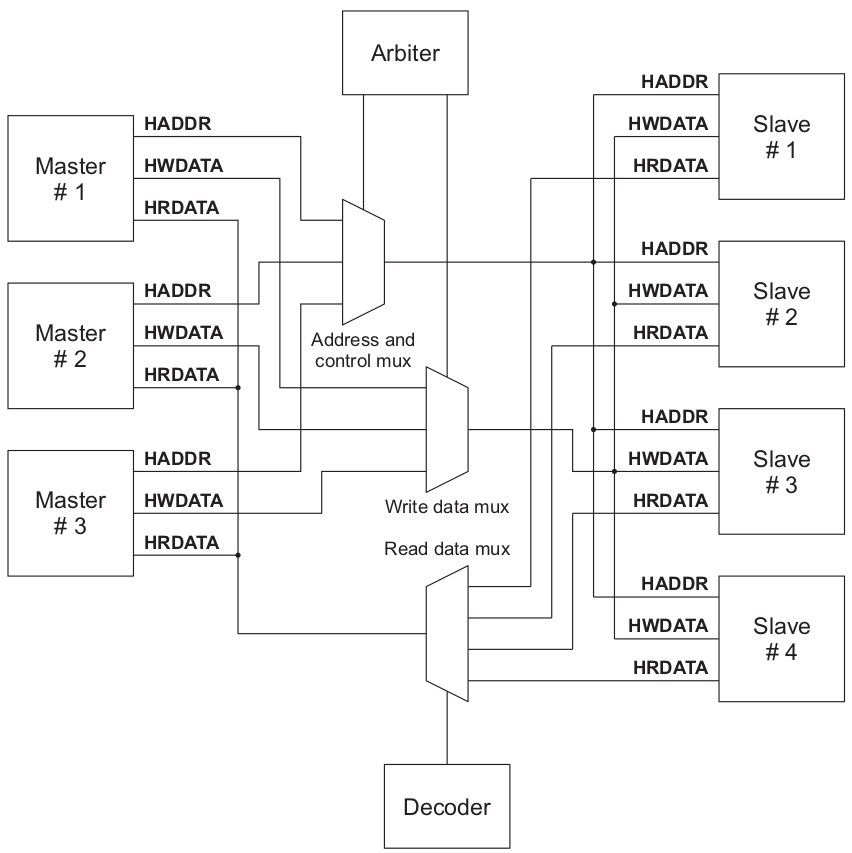
\includegraphics[width=0.8\textwidth]{figs/AHB/AHB_connections.png}
    \end{center}
    \caption{An overview of AHB interconnect, reprinted from \cite{amba}. The mux outputs are referred to as address or data buses.}
    \label{fig:interc}
\end{figure}

\newpage

\begin{figure}[hbt]
 \centering
 \begin{subfigure}[b]{0.4\linewidth}
 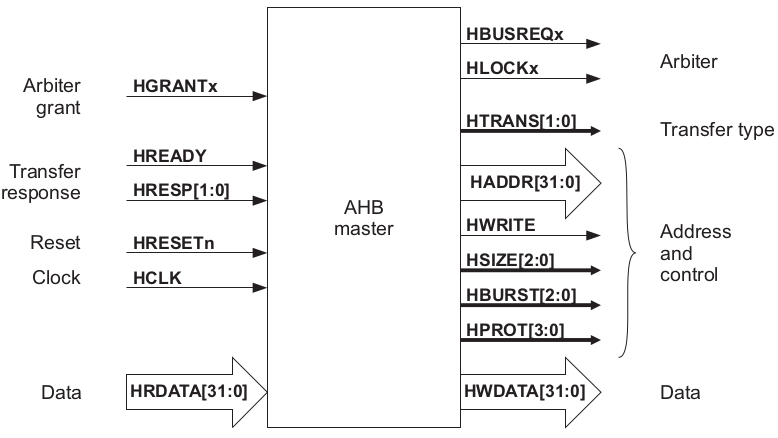
\includegraphics[width=\linewidth]{figs/AHB/master_signals.png}
 \caption{Master signals}
 \end{subfigure}
 \begin{subfigure}[b]{0.4\linewidth}
 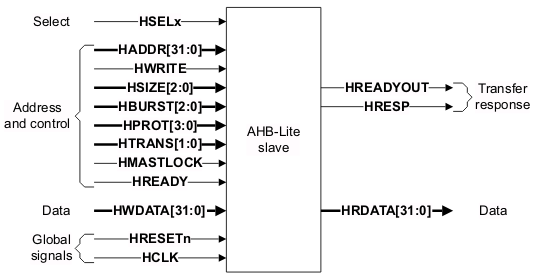
\includegraphics[width=\linewidth]{figs/AHB/slave_lite.png}
 \caption{Slave signals}
 \end{subfigure}
 \caption{Master and slave signals, reprint from left:\cite{amba} right:\cite{amba3}. AHBLite slaves are compatible with AHB systems\cite{ambacomp}. \textbf{HRESP[1:1]} is therefore hardwired to 0.}
 \label{fig:ahbsig}
\end{figure}


As figure \ref{fig:interc} illustrates, the selected address/control and data signals are broadcast to all receivers simultaneously. On the slave side every signal is ignored unless the \textbf{HSELx} signal is set by the decoder. Slave \textbf{x} then reacts to the \textbf{HTRANS[1:0]} and \textbf{HREADY} control signal. Since the master is the initiator it will only react to appropriate signals when expected. \\

\subsection{Transfers}

\subsubsection{Overview of transfer}

\TLSAY{The text below does not provide an overview ... it's very detailed. I would start with a quick overiew of read/write ... I guess you didn't end up working on burst at all? and the show the waveform and explain the hready, hreq and so on with the waveform} 
A master requests the bus by asserting its \textbf{HBUSREQx} signal. The master waits until \textbf{HREADY} and its \textbf{HGRANTx} is set and provides appropriate address and control signals in the next cycle. The transfer is now in the address phase, all set values must be kept valid until \textbf{HREADY} is set. The transfer is now in the data phase. If the transfer is a write, the master must provide valid data and keep it valid until \textbf{HREADY} is set. Otherwise it is a read, and the slave does not need to provide valid data until it sets \textbf{HREADY}. Master samples the data when \textbf{HREADY} is set.
\newpage

\begin{figure}[hbt]
    \begin{center}
        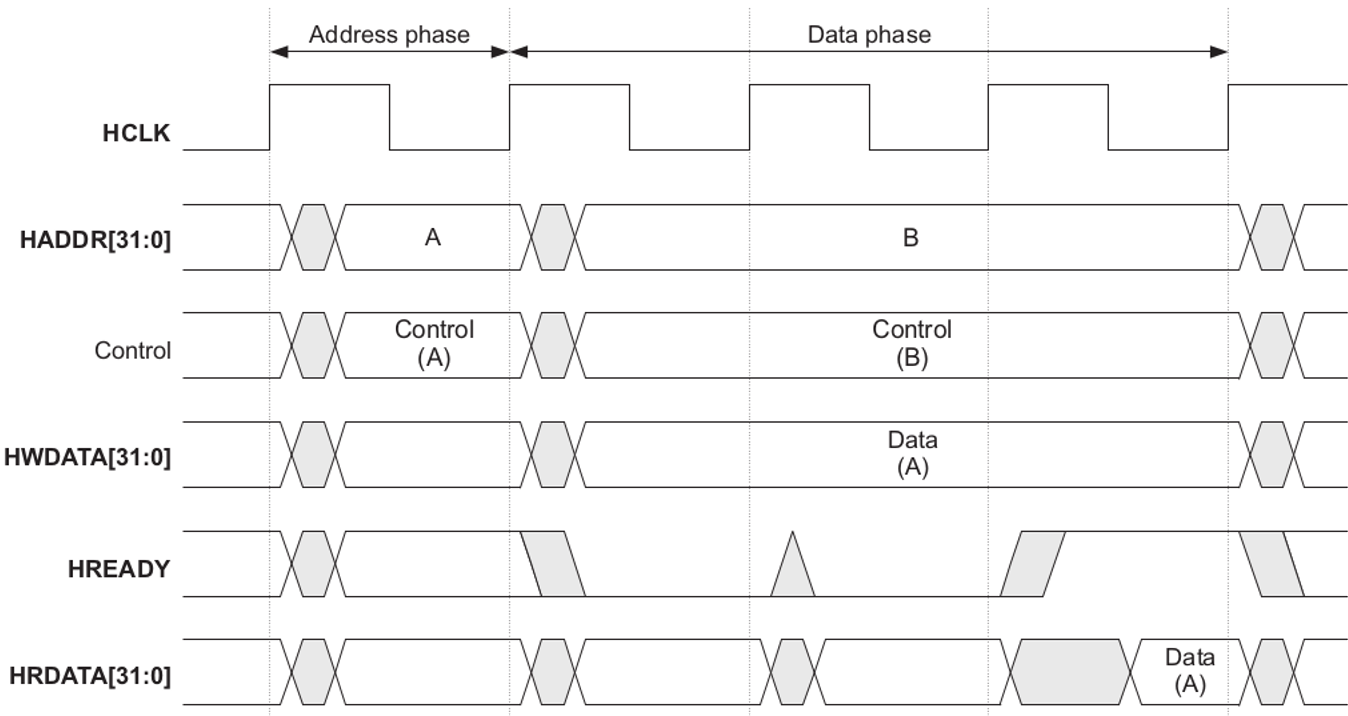
\includegraphics[width=0.8\textwidth]{figs/AHB/transfer.png}
    \end{center}
    \caption{A transfer with wait states, modified reprint from \cite{amba}. In this document the letters represent different masters}
    \label{fig:transfer}
\end{figure}

In figure \ref{fig:transfer} master A initiated a transfer, and the slave extends the data phase to give itself time to handle the request. When the slave is finished it responds using \textbf{HREADYOUT}, \textbf{HRESP} and if it is a read request, \textbf{HRDATA}, see \ref{subsubsec:slvresp}. As seen from the figure, extending the data phase for A has a side effect of extending the address phase for B. B is the address bus owner, but any selected slave knows not to react to its control signals. \textbf{HREADYOUT} is routed back to the slaves input as \textbf{HREADY} through the address mux, and must be set for the slave to sample address and control. For this reason only \textbf{HREADY} is referred to for the remainder of this document. 

\newpage
\subsection{Control signals}
The following signals determine which actions the slaves perfom:
\begin{table}[hbt]
  \label{tab:htrans}
  \begin{tabular}{|p{28mm}|r|p{10cm}|} 
  \hline
  \textbf{HTRANS[1:0]} & \textbf{Type} & \textbf{Description} \\
    \hline
  00 & \textit{idle} & No transfer required, used when a master is granted the bus but does not wish to initiate a transfer. Selected slave must always provide a zero wait state \textit{okay} response and ignore all other signals.\\
    \hline
  01 & \textit{busy} & Used by master to insert idle cycles in the middle of a burst sequence. \\
    \hline
  10 & \textit{nonseq} & Indicates the start of a transfer, address and control is unrelated to the previous transfer. Single transfers are treated as burst of one, the transfer type is therefore nonsequential\\
    \hline
  11 & \textit{seq} & The remaining transfers in a burst are sequential.\\
\hline
  \end{tabular}
\caption{Transfer type}
\end{table}

\textbf{HWRITE} indicates direction of transfer, a write request is performed when set.

\begin{table}[hbt]
  \label{tab:hsize}
  \begin{tabular}{|p{25mm}|r|p{10cm}|} 
  \hline
  \textbf{HSIZE[2:0]} & \textbf{Size} & \textbf{Description} \\
    \hline
  000 & 8 bits & \textit{Byte}\\
    \hline
  001 & 16 bits & \textit{Halfword} \\
    \hline
  010 & 32 bits & \textit{Word}\\
    \hline
  remainder & >32 bits & \textit{not implemented}.\\
\hline
  \end{tabular}
\caption{Data width}
\end{table}

\subsection{Slave responses}
\label{subsec:slvresp}
After a transfer has been started only the active slave has the ability to end it. The active uses \textbf{HREADY} in combination with \textbf{HRESP} to signal the status of the transfer. The slave can either extend and complete the transfer, or provide a two cycle error response. 

\begin{table}[hbt]
  \label{tab:hsize}
  \begin{tabular}{|r|r|p{10cm}|} 
  \hline
  \textbf{HRESP} & \textbf{HREADY} & \textbf{Description} \\
    \hline
  0 & 0 & Wait state\\
    \hline
  0 & 1 & Transfer complete/Okay response \\
    \hline
  1 & 0 & First cycle of error response\\
    \hline
  1 & 1 & Second cycle of error response \\
\hline
  \end{tabular}
\caption{Slave responses}
\end{table}

If the address provided on the address bus is outside the range of any existing slave the default slave response must be provided. If the encoding on \textbf{HTRANS[1:0]} is \textit{idle} or \textit{busy} default slave must provide a zero cycle okay response. Otherwise the default slave must provide the two cycle error response. 




